\subsection{Results for Heading}
%\label{subsec:direction_results}
%\vspace{10pt}

Figure~\ref{fig:var_direction} represents the $p$-values for the Wilcoxon signed-rank test on actual and predicted values across $k$-fold validation datasets for the heading in the $k$-fold testing datasets using different RNN models, and forecasting times. Darker colors in grayscale represent a higher $p$-value in a range from $0$ to $1$. The values on the secondary diagonal are all equal to $1$ and black because models equal themselves.

\begin{figure}[!ht]
	\centering
	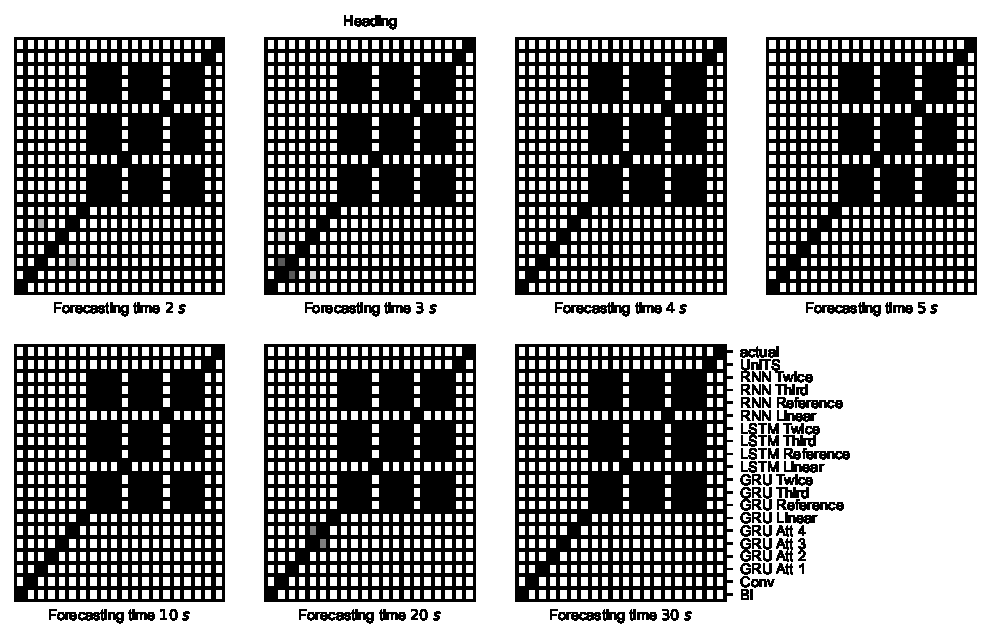
\includegraphics[width = 0.99 \linewidth]{var_direction.pdf}
	\caption{The $p$-values for the Wilcoxon signed-rank test on actual and predicted values across $k$-fold validation datasets for the heading in the $k$-fold testing datasets using different RNN models, and forecasting times. Darker colors in grayscale represent a higher $p$-value in a range from $0$ to $1$. The values on the secondary diagonal are all equal to $1$ and black because models equal themselves.}
	\label{fig:var_direction}
\end{figure}

Figure~\ref{fig:best_R2_val} contains the average $R^{2}$ (\%) across $k$-fold testing datasets using different validation datasets for all variables estimated in nested $k$-fold cross-validation by different RNN models, and forecasting times.

\begin{figure}[!ht]
	\centering
	\includegraphics[width = 0.99 \linewidth]{best_R2_val.pdf}
	\caption{The average $R^{2}$ (\%) across $k$-fold testing datasets using different validation datasets for all variables estimated in nested $k$-fold cross-validation by different RNN models, and forecasting times.}
	\label{fig:best_R2_val}
\end{figure}

The average $R^{2}$ (\%), with standard deviation in brackets, across $k$-fold validation datasets for the heading estimated on the $k$-fold testing datasets by different RNN models, and forecasting times is listed in Table~\ref{tab:best_direction_R2}.

\begin{table}[!ht]
	\centering
	\resizebox{\linewidth}{!}{
		\begin{tabular}{|c|c|c|c|c|c|c|c|}
			\hline
			Model & $2$ $s$ & $3$ $s$ & $4$ $s$ & $5$ $s$ & $10$ $s$ & $20$ $s$ & $30$ $s$ \\ \hline
			\multirow{2}{*}{Conv} & $81.67\%$ & $77.24\%$ & $\mathbf{73.59\%}$ & $\mathbf{70.18\%}$ & $57.0\%$ & $41.68\%$ & $33.83\%$ \\
			 & ($1.68\%$) & ($2.1\%$) & \textbf{(}$\mathbf{2.03\%}$\textbf{)} & \textbf{(}$\mathbf{2.35\%}$\textbf{)} & ($2.73\%$) & ($3.38\%$) & ($3.72\%$) \\ \hline
			\multirow{2}{*}{RNN Linear} & $\mathbf{86.11\%}$ & $\mathbf{79.12\%}$ & $72.83\%$ & $68.34\%$ & $51.75\%$ & $28.44\%$ & $16.2\%$ \\
			 & \textbf{(}$\mathbf{1.3\%}$\textbf{)} & \textbf{(}$\mathbf{2.11\%}$\textbf{)} & ($2.27\%$) & ($2.23\%$) & ($3.08\%$) & ($3.04\%$) & ($4.48\%$) \\ \hline
			\multirow{2}{*}{UniTS} & $77.09\%$ & $74.0\%$ & $71.12\%$ & $68.39\%$ & $\mathbf{57.72\%}$ & $\mathbf{44.0\%}$ & $\mathbf{34.98\%}$ \\
			 & ($1.99\%$) & ($2.25\%$) & ($2.42\%$) & ($2.55\%$) & \textbf{(}$\mathbf{2.76\%}$\textbf{)} & \textbf{(}$\mathbf{3.21\%}$\textbf{)} & \textbf{(}$\mathbf{3.79\%}$\textbf{)} \\ \hline
		\end{tabular}
	}
	\caption{The average $R^{2}$ (\%), with standard deviation in brackets, across $k$-fold validation datasets for the heading estimated on the $k$-fold testing datasets by different RNN models, and forecasting times.}
	\label{tab:best_direction_R2}
\end{table}

The Conv model achieved the highest $R^{2}$ (\%) for heading, and a forecasting time of $4$, and $5$ $s$ with average values and standard deviation (in brackets) that equal $73.59$\% ($2.03$\%), and $70.18$\% ($2.35$\%) respectively.

The RNN Linear model achieved the highest $R^{2}$ (\%) for heading, and a forecasting time of $2$, and $3$ $s$ with average values and standard deviation (in brackets) that equal $86.11$\% ($1.3$\%), and $79.12$\% ($2.11$\%) respectively.

The UniTS model achieved the highest $R^{2}$ (\%) for heading, and a forecasting time of $10$, $20$, and $30$ $s$ with average values and standard deviation (in brackets) that equal $57.72$\% ($2.76$\%), $44.0$\% ($3.21$\%), and $34.98$\% ($3.79$\%) respectively.

Figure~\ref{fig:best_MAE_val} contains the average MAE across $k$-fold testing datasets using different validation datasets for all variables estimated in nested $k$-fold cross-validation by different RNN models, and forecasting times.

\begin{figure}[!ht]
	\centering
	\includegraphics[width = 0.99 \linewidth]{best_MAE_val.pdf}
	\caption{The average MAE across $k$-fold testing datasets using different validation datasets for all variables estimated in nested $k$-fold cross-validation by different RNN models, and forecasting times.}
	\label{fig:best_MAE_val}
\end{figure}

The average MAE in $\degree$, with standard deviation in brackets, across $k$-fold validation datasets for the heading estimated on the $k$-fold testing datasets by different RNN models, and forecasting times is listed in Table~\ref{tab:best_direction_MAE}.

\begin{table}[!ht]
	\centering
	\resizebox{\linewidth}{!}{
		\begin{tabular}{|c|c|c|c|c|c|c|c|}
			\hline
			Model & $2$ $s$ & $3$ $s$ & $4$ $s$ & $5$ $s$ & $10$ $s$ & $20$ $s$ & $30$ $s$ \\ \hline
			\multirow{2}{*}{GRU Att 1} & $\mathbf{11.77}$ & $\mathbf{15.7}$ & $\mathbf{19.33}$ & $\mathbf{21.9}$ & $\mathbf{32.74}$ & $49.41$ & $63.77$ \\
			 & \textbf{(}$\mathbf{1.29}$\textbf{)} & \textbf{(}$\mathbf{1.63}$\textbf{)} & \textbf{(}$\mathbf{1.67}$\textbf{)} & \textbf{(}$\mathbf{1.75}$\textbf{)} & \textbf{(}$\mathbf{2.14}$\textbf{)} & ($2.48$) & ($10.68$) \\ \hline
			\multirow{2}{*}{UniTS} & $16.17$ & $19.54$ & $22.46$ & $25.04$ & $34.91$ & $\mathbf{47.49}$ & $\mathbf{55.81}$ \\
			 & ($1.21$) & ($1.41$) & ($1.56$) & ($1.68$) & ($2.0$) & \textbf{(}$\mathbf{2.55}$\textbf{)} & \textbf{(}$\mathbf{3.01}$\textbf{)} \\ \hline
		\end{tabular}
	}
	\caption{The average MAE in $\degree$, with standard deviation in brackets, across $k$-fold validation datasets for the heading estimated on the $k$-fold testing datasets by different RNN models, and forecasting times.}
	\label{tab:best_direction_MAE}
\end{table}

The GRU Att 1 model achieved the lowest MAE for heading, and a forecasting time of $10$, $2$, $3$, $4$, and $5$ $s$ with average values and standard deviation (in brackets) that equal $32.74$ $\degree$ ($2.14$ $\degree$), $11.77$ $\degree$ ($1.29$ $\degree$), $15.7$ $\degree$ ($1.63$ $\degree$), $19.33$ $\degree$ ($1.67$ $\degree$), and $21.9$ $\degree$ ($1.75$ $\degree$) respectively.

The GRU Att 1 model does not make statistically significantly different predictions than the GRU Att 4 model for heading using a forecasting time of $2$ $s$, with a $p$-value equaling $3.018 \times 10^{-1}$.

The GRU Att 1 model does not make statistically significantly different predictions than the GRU Att 3, and Conv models for heading using a forecasting time of $3$ $s$, with $p$-values equaling $4.596 \times 10^{-4}$, and $6.527 \times 10^{-1}$.

The UniTS model achieved the lowest MAE for heading, and a forecasting time of $20$, and $30$ $s$ with average values and standard deviation (in brackets) that equal $47.49$ $\degree$ ($2.55$ $\degree$), and $55.81$ $\degree$ ($3.01$ $\degree$) respectively.

\subsection{Results for $y$ Offset}
%\label{subsec:latitude_no_abs_results}
%\vspace{10pt}

Figure~\ref{fig:var_lat} represents the $p$-values for the Wilcoxon signed-rank test on actual and predicted values across $k$-fold validation datasets for the $y$ offset in the $k$-fold testing datasets using different RNN models, and forecasting times. Darker colors in grayscale represent a higher $p$-value in a range from $0$ to $1$. The values on the secondary diagonal are all equal to $1$ and black because models equal themselves.

\begin{figure}[!ht]
	\centering
	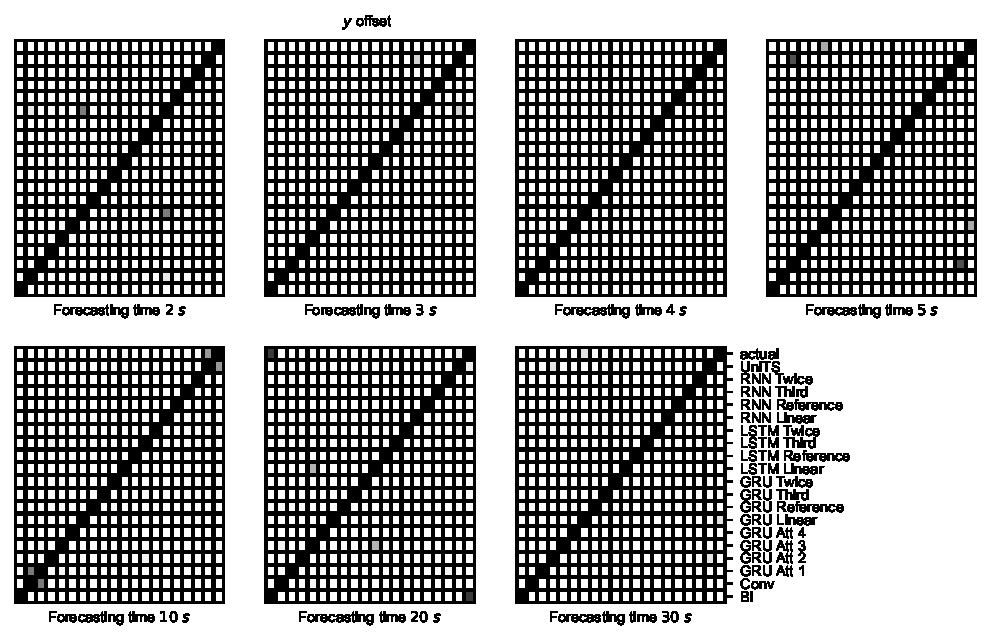
\includegraphics[width = 0.99 \linewidth]{var_lat.pdf}
	\caption{The $p$-values for the Wilcoxon signed-rank test on actual and predicted values across $k$-fold validation datasets for the $y$ offset in the $k$-fold testing datasets using different RNN models, and forecasting times. Darker colors in grayscale represent a higher $p$-value in a range from $0$ to $1$. The values on the secondary diagonal are all equal to $1$ and black because models equal themselves.}
	\label{fig:var_lat}
\end{figure}

The average $R^{2}$ (\%), with standard deviation in brackets, across $k$-fold validation datasets for the $y$ offset estimated on the $k$-fold testing datasets by different RNN models, and forecasting times is listed in Table~\ref{tab:best_latitude_no_abs_R2}.

\begin{table}[!ht]
	\centering
	\resizebox{\linewidth}{!}{
		\begin{tabular}{|c|c|c|c|c|c|c|c|}
			\hline
			Model & $2$ $s$ & $3$ $s$ & $4$ $s$ & $5$ $s$ & $10$ $s$ & $20$ $s$ & $30$ $s$ \\ \hline
			\multirow{2}{*}{Conv} & $93.52\%$ & $90.43\%$ & $86.78\%$ & $83.0\%$ & $64.03\%$ & $40.69\%$ & $\mathbf{29.8\%}$ \\
			 & ($1.09\%$) & ($1.02\%$) & ($1.17\%$) & ($1.44\%$) & ($2.07\%$) & ($2.47\%$) & \textbf{(}$\mathbf{1.4\%}$\textbf{)} \\ \hline
			\multirow{2}{*}{GRU Att 2} & $93.23\%$ & $90.0\%$ & $\mathbf{87.69\%}$ & $\mathbf{84.05\%}$ & $61.6\%$ & $28.71\%$ & $2.39\%$ \\
			 & ($1.51\%$) & ($2.05\%$) & \textbf{(}$\mathbf{1.72\%}$\textbf{)} & \textbf{(}$\mathbf{1.93\%}$\textbf{)} & ($3.4\%$) & ($6.2\%$) & ($8.4\%$) \\ \hline
			\multirow{2}{*}{GRU Reference} & $\mathbf{95.61\%}$ & $87.54\%$ & $80.31\%$ & $74.42\%$ & $45.82\%$ & $2.42\%$ & $-20.58\%$ \\
			 & \textbf{(}$\mathbf{2.14\%}$\textbf{)} & ($4.07\%$) & ($4.96\%$) & ($4.09\%$) & ($4.34\%$) & ($5.99\%$) & ($7.07\%$) \\ \hline
			\multirow{2}{*}{LSTM Third} & $93.81\%$ & $\mathbf{90.91\%}$ & $82.5\%$ & $77.25\%$ & $46.06\%$ & $1.72\%$ & $-20.76\%$ \\
			 & ($3.93\%$) & \textbf{(}$\mathbf{5.23\%}$\textbf{)} & ($8.75\%$) & ($5.43\%$) & ($3.94\%$) & ($5.94\%$) & ($9.82\%$) \\ \hline
			\multirow{2}{*}{UniTS} & $92.75\%$ & $89.96\%$ & $86.92\%$ & $83.77\%$ & $\mathbf{68.0\%}$ & $\mathbf{41.68\%}$ & $24.17\%$ \\
			 & ($1.98\%$) & ($1.67\%$) & ($1.63\%$) & ($1.67\%$) & \textbf{(}$\mathbf{2.31\%}$\textbf{)} & \textbf{(}$\mathbf{3.95\%}$\textbf{)} & ($4.68\%$) \\ \hline
		\end{tabular}
	}
	\caption{The average $R^{2}$ (\%), with standard deviation in brackets, across $k$-fold validation datasets for the $y$ offset estimated on the $k$-fold testing datasets by different RNN models, and forecasting times.}
	\label{tab:best_latitude_no_abs_R2}
\end{table}

The Conv model achieved the highest $R^{2}$ (\%) for $y$ offset, and a forecasting time of $30$ $s$ with an average value and standard deviation (in brackets) that equals $29.8$\% ($1.4$\%).

The GRU Att 2 model achieved the highest $R^{2}$ (\%) for $y$ offset, and a forecasting time of $4$, and $5$ $s$ with average values and standard deviation (in brackets) that equal $87.69$\% ($1.72$\%), and $84.05$\% ($1.93$\%) respectively.

The GRU Att 2 model does not make statistically significantly different predictions than the GRU Att 3 model for $y$ offset using a forecasting time of $4$ $s$, with a $p$-value equaling $2.656 \times 10^{-4}$.

The GRU Reference model achieved the highest $R^{2}$ (\%) for $y$ offset, and a forecasting time of $2$ $s$ with an average value and standard deviation (in brackets) that equals $95.61$\% ($2.14$\%).

The LSTM Third model achieved the highest $R^{2}$ (\%) for $y$ offset, and a forecasting time of $3$ $s$ with an average value and standard deviation (in brackets) that equals $90.91$\% ($5.23$\%).

The LSTM Third model does not make statistically significantly different predictions than the LSTM Twice model for $y$ offset using a forecasting time of $3$ $s$, with a $p$-value equaling $6.104 \times 10^{-2}$.

The UniTS model achieved the highest $R^{2}$ (\%) for $y$ offset, and a forecasting time of $10$, and $20$ $s$ with average values and standard deviation (in brackets) that equal $68.0$\% ($2.31$\%), and $41.68$\% ($3.95$\%) respectively.

The UniTS model does not make statistically significantly different predictions than the GRU Att 3, and actual value models for $y$ offset using a forecasting time of $10$ $s$, with $p$-values equaling $7.389 \times 10^{-3}$, and $4.075 \times 10^{-1}$.

The UniTS model does not make statistically significantly different predictions than the actual value, and Bi models for $y$ offset using a forecasting time of $20$ $s$, with $p$-values equaling $6.866 \times 10^{-2}$, and $1.408 \times 10^{-3}$.

The average MAE in $\degree$ ($\times 10^{-5}$), with standard deviation in brackets, across $k$-fold validation datasets for the $y$ offset estimated on the $k$-fold testing datasets by different RNN models, and forecasting times is listed in Table~\ref{tab:best_latitude_no_abs_MAE}.

\begin{table}[!ht]
	\centering
	\resizebox{\linewidth}{!}{
		\begin{tabular}{|c|c|c|c|c|c|c|c|}
			\hline
			Model & $2$ $s$ & $3$ $s$ & $4$ $s$ & $5$ $s$ & $10$ $s$ & $20$ $s$ & $30$ $s$ \\ \hline
			\multirow{2}{*}{GRU Att 1} & $\mathbf{5.558}$ & $\mathbf{7.454}$ & $8.885$ & $10.171$ & $20.701$ & $28.391$ & $32.677$ \\
			 & \textbf{(}$\mathbf{0.492}$\textbf{)} & \textbf{(}$\mathbf{0.708}$\textbf{)} & ($0.707$) & ($0.941$) & ($4.684$) & ($3.632$) & ($2.745$) \\ \hline
			\multirow{2}{*}{GRU Att 2} & $6.187$ & $7.917$ & $\mathbf{8.816}$ & $\mathbf{10.118}$ & $16.546$ & $23.948$ & $29.776$ \\
			 & ($0.608$) & ($1.082$) & \textbf{(}$\mathbf{0.762}$\textbf{)} & \textbf{(}$\mathbf{0.997}$\textbf{)} & ($1.513$) & ($2.1$) & ($2.891$) \\ \hline
			\multirow{2}{*}{GRU Att 4} & $5.863$ & $8.231$ & $9.942$ & $11.388$ & $\mathbf{16.223}$ & $26.774$ & $32.495$ \\
			 & ($0.526$) & ($0.708$) & ($0.854$) & ($1.044$) & \textbf{(}$\mathbf{1.953}$\textbf{)} & ($4.307$) & ($3.099$) \\ \hline
			\multirow{2}{*}{UniTS} & $7.176$ & $8.763$ & $10.181$ & $11.466$ & $16.562$ & $\mathbf{23.209}$ & $\mathbf{27.355}$ \\
			 & ($0.607$) & ($0.759$) & ($0.88$) & ($0.988$) & ($1.426$) & \textbf{(}$\mathbf{2.001}$\textbf{)} & \textbf{(}$\mathbf{2.3}$\textbf{)} \\ \hline
		\end{tabular}
	}
	\caption{The average MAE in $\degree$ ($\times 10^{-5}$), with standard deviation in brackets, across $k$-fold validation datasets for the $y$ offset estimated on the $k$-fold testing datasets by different RNN models, and forecasting times.}
	\label{tab:best_latitude_no_abs_MAE}
\end{table}

The GRU Att 1 model achieved the lowest MAE for $y$ offset, and a forecasting time of $2$, and $3$ $s$ with average values and standard deviation (in brackets) that equal $5.558 \times 10^{-5}$ $\degree$ ($0.492 \times 10^{-5}$ $\degree$), and $7.454 \times 10^{-5}$ $\degree$ ($0.708 \times 10^{-5}$ $\degree$) respectively.

The GRU Att 1 model does not make statistically significantly different predictions than the UniTS model for $y$ offset using a forecasting time of $2$ $s$, with a $p$-value equaling $1.373 \times 10^{-3}$.

The GRU Att 2 model achieved the lowest MAE for $y$ offset, and a forecasting time of $4$, and $5$ $s$ with average values and standard deviation (in brackets) that equal $8.816 \times 10^{-5}$ $\degree$ ($0.762 \times 10^{-5}$ $\degree$), and $10.118 \times 10^{-5}$ $\degree$ ($0.997 \times 10^{-5}$ $\degree$) respectively.

The GRU Att 2 model does not make statistically significantly different predictions than the GRU Att 3 model for $y$ offset using a forecasting time of $4$ $s$, with a $p$-value equaling $2.656 \times 10^{-4}$.

The GRU Att 4 model achieved the lowest MAE for $y$ offset, and a forecasting time of $10$ $s$ with an average value and standard deviation (in brackets) that equals $16.223 \times 10^{-5}$ $\degree$ ($1.953 \times 10^{-5}$ $\degree$).

The GRU Att 4 model does not make statistically significantly different predictions than the LSTM Linear model for $y$ offset using a forecasting time of $10$ $s$, with a $p$-value equaling $1.121 \times 10^{-2}$.

The UniTS model achieved the lowest MAE for $y$ offset, and a forecasting time of $20$, and $30$ $s$ with average values and standard deviation (in brackets) that equal $23.209 \times 10^{-5}$ $\degree$ ($2.001 \times 10^{-5}$ $\degree$), and $27.355 \times 10^{-5}$ $\degree$ ($2.3 \times 10^{-5}$ $\degree$) respectively.

The UniTS model does not make statistically significantly different predictions than the actual value, and Bi models for $y$ offset using a forecasting time of $20$ $s$, with $p$-values equaling $6.866 \times 10^{-2}$, and $1.408 \times 10^{-3}$.

The UniTS model does not make statistically significantly different predictions than the GRU Att 2, GRU Linear, and actual value models for $y$ offset using a forecasting time of $30$ $s$, with $p$-values equaling $1.002 \times 10^{-1}$, $3.812 \times 10^{-3}$, and $1.084 \times 10^{-2}$.

\subsection{Results for $x$ Offset}
%\label{subsec:longitude_no_abs_results}
%\vspace{10pt}

Figure~\ref{fig:var_long} represents the $p$-values for the Wilcoxon signed-rank test on actual and predicted values across $k$-fold validation datasets for the $x$ offset in the $k$-fold testing datasets using different RNN models, and forecasting times. Darker colors in grayscale represent a higher $p$-value in a range from $0$ to $1$. The values on the secondary diagonal are all equal to $1$ and black because models equal themselves.

\begin{figure}[!ht]
	\centering
	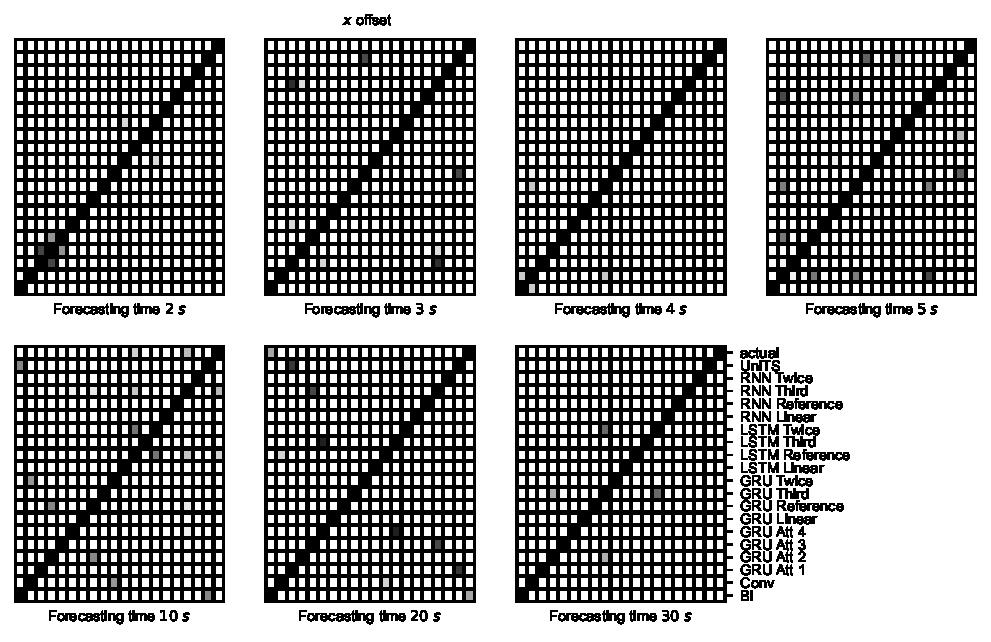
\includegraphics[width = 0.99 \linewidth]{var_long.pdf}
	\caption{The $p$-values for the Wilcoxon signed-rank test on actual and predicted values across $k$-fold validation datasets for the $x$ offset in the $k$-fold testing datasets using different RNN models, and forecasting times. Darker colors in grayscale represent a higher $p$-value in a range from $0$ to $1$. The values on the secondary diagonal are all equal to $1$ and black because models equal themselves.}
	\label{fig:var_long}
\end{figure}

The average $R^{2}$ (\%), with standard deviation in brackets, across $k$-fold validation datasets for the $x$ offset estimated on the $k$-fold testing datasets by different RNN models, and forecasting times is listed in Table~\ref{tab:best_longitude_no_abs_R2}.

\begin{table}[!ht]
	\centering
	\resizebox{\linewidth}{!}{
		\begin{tabular}{|c|c|c|c|c|c|c|c|}
			\hline
			Model & $2$ $s$ & $3$ $s$ & $4$ $s$ & $5$ $s$ & $10$ $s$ & $20$ $s$ & $30$ $s$ \\ \hline
			\multirow{2}{*}{Bi} & $94.51\%$ & $91.31\%$ & $87.8\%$ & $84.03\%$ & $66.95\%$ & $\mathbf{43.14\%}$ & $\mathbf{29.73\%}$ \\
			 & ($0.79\%$) & ($1.3\%$) & ($1.64\%$) & ($1.75\%$) & ($2.53\%$) & \textbf{(}$\mathbf{2.76\%}$\textbf{)} & \textbf{(}$\mathbf{3.03\%}$\textbf{)} \\ \hline
			\multirow{2}{*}{GRU Att 1} & $95.29\%$ & $\mathbf{91.83\%}$ & $87.74\%$ & $84.62\%$ & $50.34\%$ & $14.63\%$ & $3.01\%$ \\
			 & ($0.92\%$) & \textbf{(}$\mathbf{1.53\%}$\textbf{)} & ($2.02\%$) & ($2.12\%$) & ($14.06\%$) & ($5.96\%$) & ($13.0\%$) \\ \hline
			\multirow{2}{*}{LSTM Third} & $\mathbf{96.88\%}$ & $89.96\%$ & $83.59\%$ & $76.3\%$ & $47.76\%$ & $-0.74\%$ & $-22.31\%$ \\
			 & \textbf{(}$\mathbf{1.13\%}$\textbf{)} & ($3.73\%$) & ($4.38\%$) & ($4.29\%$) & ($4.45\%$) & ($5.66\%$) & ($4.66\%$) \\ \hline
			\multirow{2}{*}{UniTS} & $93.99\%$ & $91.18\%$ & $\mathbf{88.19\%}$ & $\mathbf{85.09\%}$ & $\mathbf{69.54\%}$ & $42.6\%$ & $23.39\%$ \\
			 & ($0.83\%$) & ($1.05\%$) & \textbf{(}$\mathbf{1.32\%}$\textbf{)} & \textbf{(}$\mathbf{1.57\%}$\textbf{)} & \textbf{(}$\mathbf{2.54\%}$\textbf{)} & ($3.68\%$) & ($4.0\%$) \\ \hline
		\end{tabular}
	}
	\caption{The average $R^{2}$ (\%), with standard deviation in brackets, across $k$-fold validation datasets for the $x$ offset estimated on the $k$-fold testing datasets by different RNN models, and forecasting times.}
	\label{tab:best_longitude_no_abs_R2}
\end{table}

The Bi model achieved the highest $R^{2}$ (\%) for $x$ offset, and a forecasting time of $20$, and $30$ $s$ with average values and standard deviation (in brackets) that equal $43.14$\% ($2.76$\%), and $29.73$\% ($3.03$\%) respectively.

The Bi model does not make statistically significantly different predictions than the actual value model for $x$ offset using a forecasting time of $20$ $s$, with a $p$-value equaling $3.471 \times 10^{-1}$.

The GRU Att 1 model achieved the highest $R^{2}$ (\%) for $x$ offset, and a forecasting time of $3$ $s$ with an average value and standard deviation (in brackets) that equals $91.83$\% ($1.53$\%).

The GRU Att 1 model does not make statistically significantly different predictions than the GRU Att 4, and RNN Third models for $x$ offset using a forecasting time of $3$ $s$, with $p$-values equaling $1.579 \times 10^{-1}$, and $8.207 \times 10^{-1}$.

The LSTM Third model achieved the highest $R^{2}$ (\%) for $x$ offset, and a forecasting time of $2$ $s$ with an average value and standard deviation (in brackets) that equals $96.88$\% ($1.13$\%).

The UniTS model achieved the highest $R^{2}$ (\%) for $x$ offset, and a forecasting time of $4$, $5$, and $10$ $s$ with average values and standard deviation (in brackets) that equal $88.19$\% ($1.32$\%), $85.09$\% ($1.57$\%), and $69.54$\% ($2.54$\%) respectively.

The UniTS model does not make statistically significantly different predictions than the GRU Twice, and LSTM Third models for $x$ offset using a forecasting time of $5$ $s$, with $p$-values equaling $6.213 \times 10^{-1}$, and $2.591 \times 10^{-1}$.

The UniTS model does not make statistically significantly different predictions than the RNN Third, and Bi models for $x$ offset using a forecasting time of $10$ $s$, with $p$-values equaling $1.747 \times 10^{-3}$, and $4.766 \times 10^{-1}$.

The average MAE in $\degree$ ($\times 10^{-5}$), with standard deviation in brackets, across $k$-fold validation datasets for the $x$ offset estimated on the $k$-fold testing datasets by different RNN models, and forecasting times is listed in Table~\ref{tab:best_longitude_no_abs_MAE}.

\begin{table}[!ht]
	\centering
	\resizebox{\linewidth}{!}{
		\begin{tabular}{|c|c|c|c|c|c|c|c|}
			\hline
			Model & $2$ $s$ & $3$ $s$ & $4$ $s$ & $5$ $s$ & $10$ $s$ & $20$ $s$ & $30$ $s$ \\ \hline
			\multirow{2}{*}{GRU Att 1} & $\mathbf{6.81}$ & $\mathbf{9.13}$ & $\mathbf{11.39}$ & $\mathbf{12.77}$ & $25.31$ & $37.95$ & $42.58$ \\
			 & \textbf{(}$\mathbf{0.85}$\textbf{)} & \textbf{(}$\mathbf{1.09}$\textbf{)} & \textbf{(}$\mathbf{1.48}$\textbf{)} & \textbf{(}$\mathbf{1.41}$\textbf{)} & ($5.26$) & ($3.28$) & ($3.71$) \\ \hline
			\multirow{2}{*}{GRU Att 2} & $7.15$ & $9.67$ & $11.58$ & $13.14$ & $\mathbf{20.61}$ & $31.95$ & $40.63$ \\
			 & ($0.86$) & ($1.3$) & ($1.44$) & ($2.01$) & \textbf{(}$\mathbf{2.81}$\textbf{)} & ($3.97$) & ($4.81$) \\ \hline
			\multirow{2}{*}{UniTS} & $9.01$ & $11.04$ & $12.85$ & $14.49$ & $21.05$ & $\mathbf{29.73}$ & $\mathbf{35.17}$ \\
			 & ($0.96$) & ($1.19$) & ($1.38$) & ($1.55$) & ($2.2$) & \textbf{(}$\mathbf{3.04}$\textbf{)} & \textbf{(}$\mathbf{3.37}$\textbf{)} \\ \hline
		\end{tabular}
	}
	\caption{The average MAE in $\degree$ ($\times 10^{-5}$), with standard deviation in brackets, across $k$-fold validation datasets for the $x$ offset estimated on the $k$-fold testing datasets by different RNN models, and forecasting times.}
	\label{tab:best_longitude_no_abs_MAE}
\end{table}

The GRU Att 1 model achieved the lowest MAE for $x$ offset, and a forecasting time of $2$, $3$, $4$, and $5$ $s$ with average values and standard deviation (in brackets) that equal $6.81 \times 10^{-5}$ $\degree$ ($0.85 \times 10^{-5}$ $\degree$), $9.13 \times 10^{-5}$ $\degree$ ($1.09 \times 10^{-5}$ $\degree$), $11.39 \times 10^{-5}$ $\degree$ ($1.48 \times 10^{-5}$ $\degree$), and $12.77 \times 10^{-5}$ $\degree$ ($1.41 \times 10^{-5}$ $\degree$) respectively.

The GRU Att 1 model does not make statistically significantly different predictions than the GRU Att 2, and GRU Att 3 models for $x$ offset using a forecasting time of $2$ $s$, with $p$-values equaling $7.278 \times 10^{-1}$, and $2.838 \times 10^{-2}$.

The GRU Att 1 model does not make statistically significantly different predictions than the GRU Att 4, and RNN Third models for $x$ offset using a forecasting time of $3$ $s$, with $p$-values equaling $1.579 \times 10^{-1}$, and $8.207 \times 10^{-1}$.

The GRU Att 1 model does not make statistically significantly different predictions than the RNN Linear, and Bi models for $x$ offset using a forecasting time of $4$ $s$, with $p$-values equaling $2.789 \times 10^{-2}$, and $3.721 \times 10^{-3}$.

The GRU Att 1 model does not make statistically significantly different predictions than the Conv model for $x$ offset using a forecasting time of $5$ $s$, with a $p$-value equaling $5.193 \times 10^{-2}$.

The GRU Att 2 model achieved the lowest MAE for $x$ offset, and a forecasting time of $10$ $s$ with an average value and standard deviation (in brackets) that equals $20.61 \times 10^{-5}$ $\degree$ ($2.81 \times 10^{-5}$ $\degree$).

The GRU Att 2 model does not make statistically significantly different predictions than the GRU Reference, and Bi models for $x$ offset using a forecasting time of $10$ $s$, with $p$-values equaling $4.694 \times 10^{-1}$, and $1.319 \times 10^{-2}$.

The UniTS model achieved the lowest MAE for $x$ offset, and a forecasting time of $20$, and $30$ $s$ with average values and standard deviation (in brackets) that equal $29.73 \times 10^{-5}$ $\degree$ ($3.04 \times 10^{-5}$ $\degree$), and $35.17 \times 10^{-5}$ $\degree$ ($3.37 \times 10^{-5}$ $\degree$) respectively.

The UniTS model does not make statistically significantly different predictions than the GRU Att 1, and LSTM Twice models for $x$ offset using a forecasting time of $20$ $s$, with $p$-values equaling $7.814 \times 10^{-1}$, and $5.546 \times 10^{-2}$.

The UniTS model does not make statistically significantly different predictions than the GRU Reference model for $x$ offset using a forecasting time of $30$ $s$, with a $p$-value equaling $6.734 \times 10^{-3}$.

\subsection{Results for Speed}
%\label{subsec:speed_results}
%\vspace{10pt}

Figure~\ref{fig:var_speed} represents the $p$-values for the Wilcoxon signed-rank test on actual and predicted values across $k$-fold validation datasets for the speed in the $k$-fold testing datasets using different RNN models, and forecasting times. Darker colors in grayscale represent a higher $p$-value in a range from $0$ to $1$. The values on the secondary diagonal are all equal to $1$ and black because models equal themselves.

\begin{figure}[!ht]
	\centering
	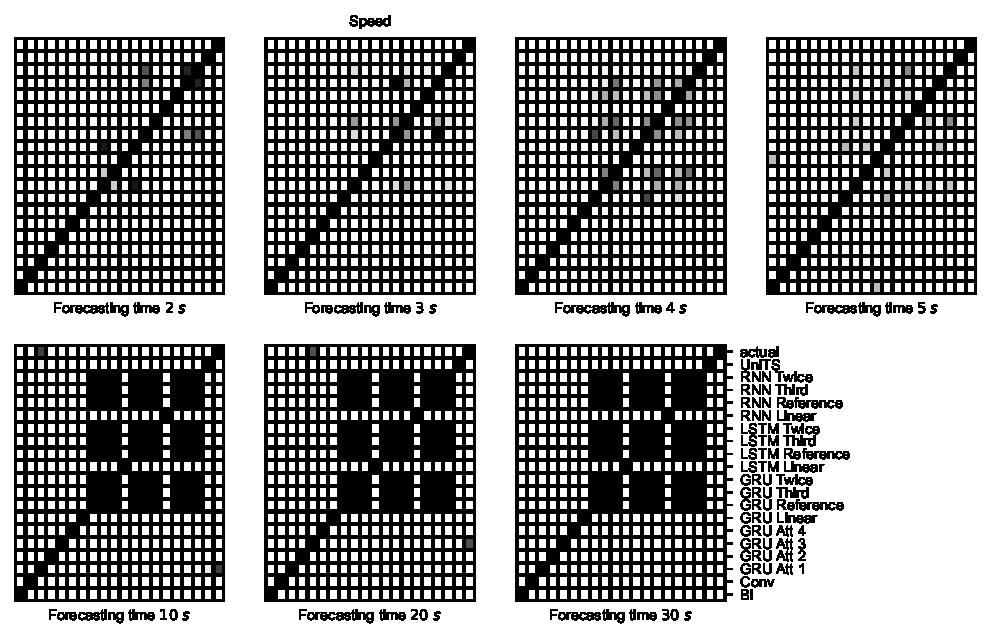
\includegraphics[width = 0.99 \linewidth]{var_speed.pdf}
	\caption{The $p$-values for the Wilcoxon signed-rank test on actual and predicted values across $k$-fold validation datasets for the speed in the $k$-fold testing datasets using different RNN models, and forecasting times. Darker colors in grayscale represent a higher $p$-value in a range from $0$ to $1$. The values on the secondary diagonal are all equal to $1$ and black because models equal themselves.}
	\label{fig:var_speed}
\end{figure}

The average $R^{2}$ (\%), with standard deviation in brackets, across $k$-fold validation datasets for the speed estimated on the $k$-fold testing datasets by different RNN models, and forecasting times is listed in Table~\ref{tab:best_speed_R2}.

\begin{table}[!ht]
	\centering
	\resizebox{\linewidth}{!}{
		\begin{tabular}{|c|c|c|c|c|c|c|c|}
			\hline
			Model & $2$ $s$ & $3$ $s$ & $4$ $s$ & $5$ $s$ & $10$ $s$ & $20$ $s$ & $30$ $s$ \\ \hline
			\multirow{2}{*}{Conv} & $94.0\%$ & $\mathbf{90.63\%}$ & $87.03\%$ & $83.37\%$ & $69.34\%$ & $55.82\%$ & $49.88\%$ \\
			 & ($0.66\%$) & \textbf{(}$\mathbf{1.04\%}$\textbf{)} & ($1.31\%$) & ($1.44\%$) & ($2.59\%$) & ($3.81\%$) & ($3.84\%$) \\ \hline
			\multirow{2}{*}{LSTM Linear} & $\mathbf{94.39\%}$ & $89.11\%$ & $83.69\%$ & $78.54\%$ & $62.8\%$ & $54.98\%$ & $51.44\%$ \\
			 & \textbf{(}$\mathbf{0.63\%}$\textbf{)} & ($1.3\%$) & ($1.83\%$) & ($2.27\%$) & ($3.95\%$) & ($4.2\%$) & ($4.16\%$) \\ \hline
			\multirow{2}{*}{UniTS} & $93.45\%$ & $90.5\%$ & $\mathbf{87.48\%}$ & $\mathbf{84.54\%}$ & $\mathbf{72.89\%}$ & $\mathbf{61.53\%}$ & $\mathbf{56.21\%}$ \\
			 & ($0.64\%$) & ($0.92\%$) & \textbf{(}$\mathbf{1.21\%}$\textbf{)} & \textbf{(}$\mathbf{1.49\%}$\textbf{)} & \textbf{(}$\mathbf{2.68\%}$\textbf{)} & \textbf{(}$\mathbf{3.89\%}$\textbf{)} & \textbf{(}$\mathbf{3.92\%}$\textbf{)} \\ \hline
		\end{tabular}
	}
	\caption{The average $R^{2}$ (\%), with standard deviation in brackets, across $k$-fold validation datasets for the speed estimated on the $k$-fold testing datasets by different RNN models, and forecasting times.}
	\label{tab:best_speed_R2}
\end{table}

The Conv model achieved the highest $R^{2}$ (\%) for speed, and a forecasting time of $3$ $s$ with an average value and standard deviation (in brackets) that equals $90.63$\% ($1.04$\%).

The LSTM Linear model achieved the highest $R^{2}$ (\%) for speed, and a forecasting time of $2$ $s$ with an average value and standard deviation (in brackets) that equals $94.39$\% ($0.63$\%).

The LSTM Linear model does not make statistically significantly different predictions than the GRU Linear model for speed using a forecasting time of $2$ $s$, with a $p$-value equaling $5.067 \times 10^{-4}$.

The UniTS model achieved the highest $R^{2}$ (\%) for speed, and a forecasting time of $4$, $5$, $10$, $20$, and $30$ $s$ with average values and standard deviation (in brackets) that equal $87.48$\% ($1.21$\%), $84.54$\% ($1.49$\%), $72.89$\% ($2.68$\%), $61.53$\% ($3.89$\%), and $56.21$\% ($3.92$\%) respectively.

The UniTS model does not make statistically significantly different predictions than the GRU Att 1 model for speed using a forecasting time of $10$ $s$, with a $p$-value equaling $7.354 \times 10^{-2}$.

The average MAE in $km/h$, with standard deviation in brackets, across $k$-fold validation datasets for the speed estimated on the $k$-fold testing datasets by different RNN models, and forecasting times is listed in Table~\ref{tab:best_speed_MAE}.

\begin{table}[!ht]
	\centering
	\resizebox{\linewidth}{!}{
		\begin{tabular}{|c|c|c|c|c|c|c|c|}
			\hline
			Model & $2$ $s$ & $3$ $s$ & $4$ $s$ & $5$ $s$ & $10$ $s$ & $20$ $s$ & $30$ $s$ \\ \hline
			\multirow{2}{*}{Conv} & $2.7$ & $\mathbf{3.29}$ & $3.91$ & $4.43$ & $6.22$ & $7.86$ & $8.56$ \\
			 & ($0.25$) & \textbf{(}$\mathbf{0.31}$\textbf{)} & ($0.37$) & ($0.42$) & ($0.56$) & ($0.61$) & ($0.69$) \\ \hline
			\multirow{2}{*}{LSTM Linear} & $\mathbf{2.46}$ & $3.42$ & $4.22$ & $4.87$ & $6.77$ & $7.92$ & $8.46$ \\
			 & \textbf{(}$\mathbf{0.23}$\textbf{)} & ($0.34$) & ($0.43$) & ($0.45$) & ($0.56$) & ($0.59$) & ($0.67$) \\ \hline
			\multirow{2}{*}{UniTS} & $2.76$ & $3.31$ & $\mathbf{3.8}$ & $\mathbf{4.23}$ & $\mathbf{5.7}$ & $\mathbf{7.02}$ & $\mathbf{7.65}$ \\
			 & ($0.26$) & ($0.31$) & \textbf{(}$\mathbf{0.36}$\textbf{)} & \textbf{(}$\mathbf{0.4}$\textbf{)} & \textbf{(}$\mathbf{0.55}$\textbf{)} & \textbf{(}$\mathbf{0.66}$\textbf{)} & \textbf{(}$\mathbf{0.67}$\textbf{)} \\ \hline
		\end{tabular}
	}
	\caption{The average MAE in $km/h$, with standard deviation in brackets, across $k$-fold validation datasets for the speed estimated on the $k$-fold testing datasets by different RNN models, and forecasting times.}
	\label{tab:best_speed_MAE}
\end{table}

The Conv model achieved the lowest MAE for speed, and a forecasting time of $3$ $s$ with an average value and standard deviation (in brackets) that equals $3.29$ $km/h$ ($0.31$ $km/h$).

The LSTM Linear model achieved the lowest MAE for speed, and a forecasting time of $2$ $s$ with an average value and standard deviation (in brackets) that equals $2.46$ $km/h$ ($0.23$ $km/h$).

The LSTM Linear model does not make statistically significantly different predictions than the GRU Linear model for speed using a forecasting time of $2$ $s$, with a $p$-value equaling $5.067 \times 10^{-4}$.

The UniTS model achieved the lowest MAE for speed, and a forecasting time of $4$, $5$, $10$, $20$, and $30$ $s$ with average values and standard deviation (in brackets) that equal $3.8$ $km/h$ ($0.36$ $km/h$), $4.23$ $km/h$ ($0.4$ $km/h$), $5.7$ $km/h$ ($0.55$ $km/h$), $7.02$ $km/h$ ($0.66$ $km/h$), and $7.65$ $km/h$ ($0.67$ $km/h$) respectively.

The UniTS model does not make statistically significantly different predictions than the GRU Att 1 model for speed using a forecasting time of $10$ $s$, with a $p$-value equaling $7.354 \times 10^{-2}$.

